\subsubsection{Speech Recognition}
Most speech patterns can be broken down into basic parts. We know these familiar parts as syllables of speech. These discrete sections of words can be combined together to form long strings of sentences. For our case, these sentences are the songs of the birds. Syllables are made using a basal tone in the throat of the animal, which is then filtered by a formation of the muscles around the throat. The result is that many syllables have repetitive sound structures that, when transformed by the Fourier transform, can be modeled by HMM.\par

\begin{center}
  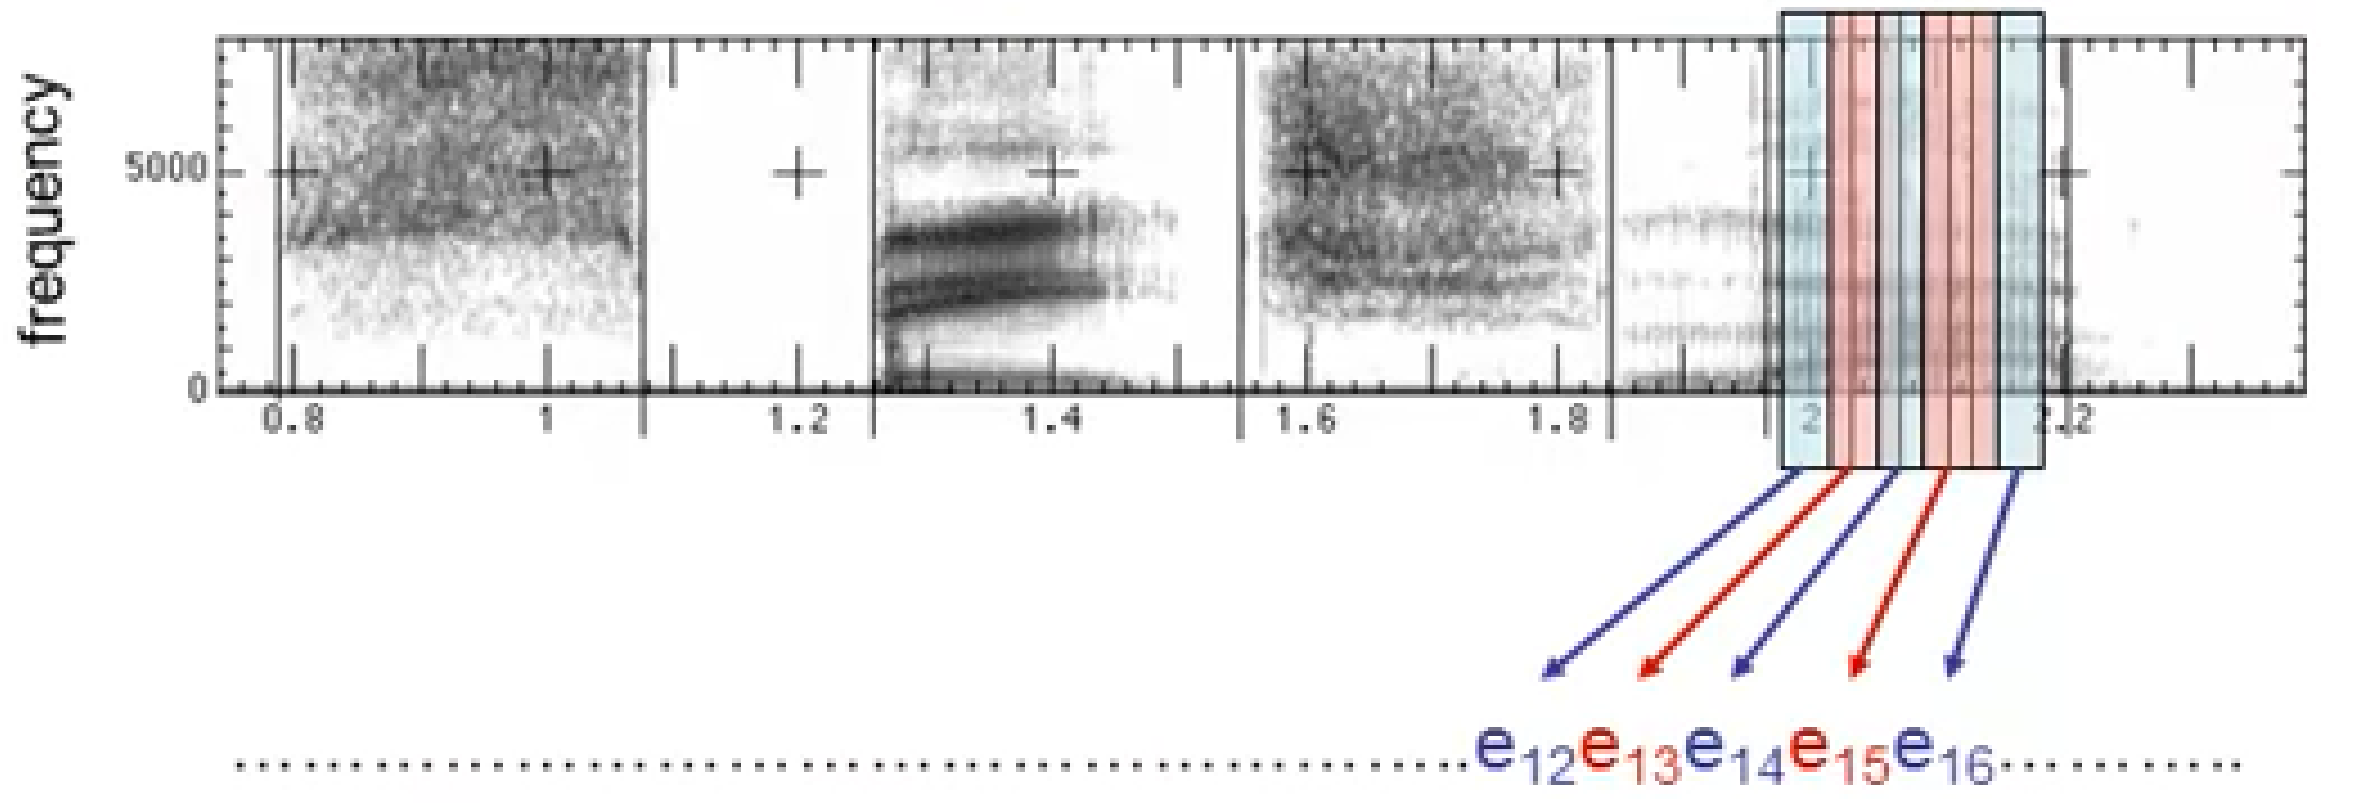
\includegraphics[width=\textwidth]{HMMSpeech}
\end{center}

For each slice of the spectrograph that we analyze, the actual sound that was emitted and transformed is the evidence. Since it is directly dependent on what syllable is being said, that same syllable is our hidden state. The state space for these states consists of all the syllables that a bird species can produce. It is easy to see why expanding this to a system that included several different types of animals would increase the state space far too much to have efficient analyses of the sounds.\par
As shown in the model below, when we enter a state space that represents the syllable, we have a probability of staying within that state space. This probability decreases as time continues, as the likelihood the syllable is still being held goes down. Within this state space, evidence is produced based on a probability model used for the specific syllable we are in. Once the probability is low enough, it becomes likely that we will move to another state space.\par

\begin{center}
  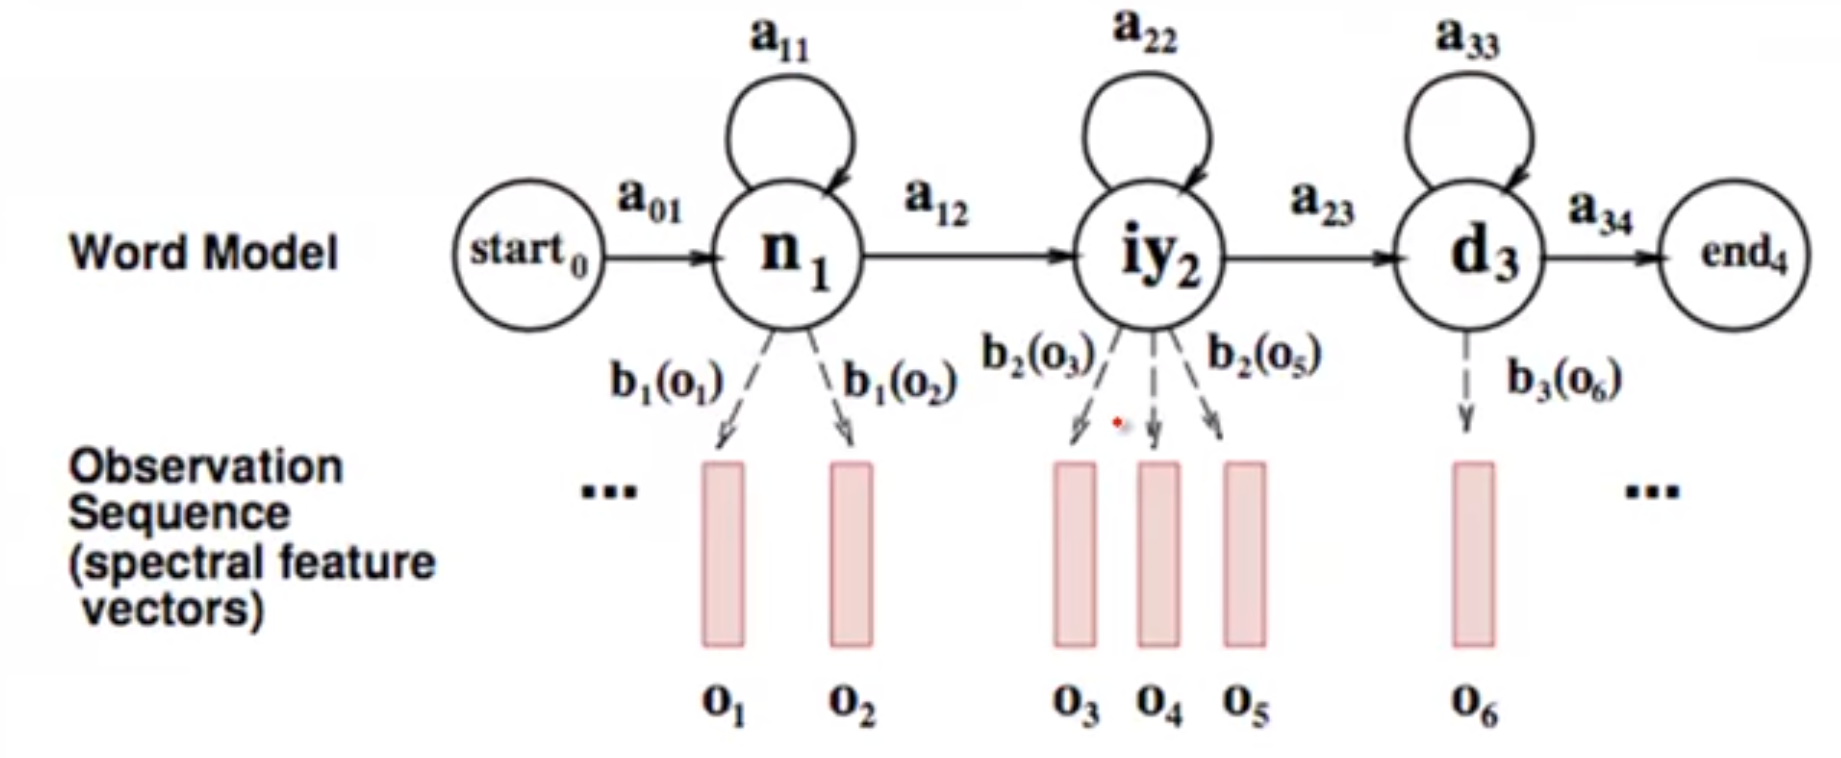
\includegraphics[width=\textwidth]{transitionModel}
\end{center}

Something further to consider would be the use of a bigram model. This model uses groupings of bird song syllables to construct ``words.'' This would allow the positioning of these words to give information on upcoming words. Much like in human languages, the use of certain words increases the chance of upcoming words. Models like these would further improve the accuracy of our analysis.
\cite{berkeley}
